\begin{figure}[!ht]
    \centering
    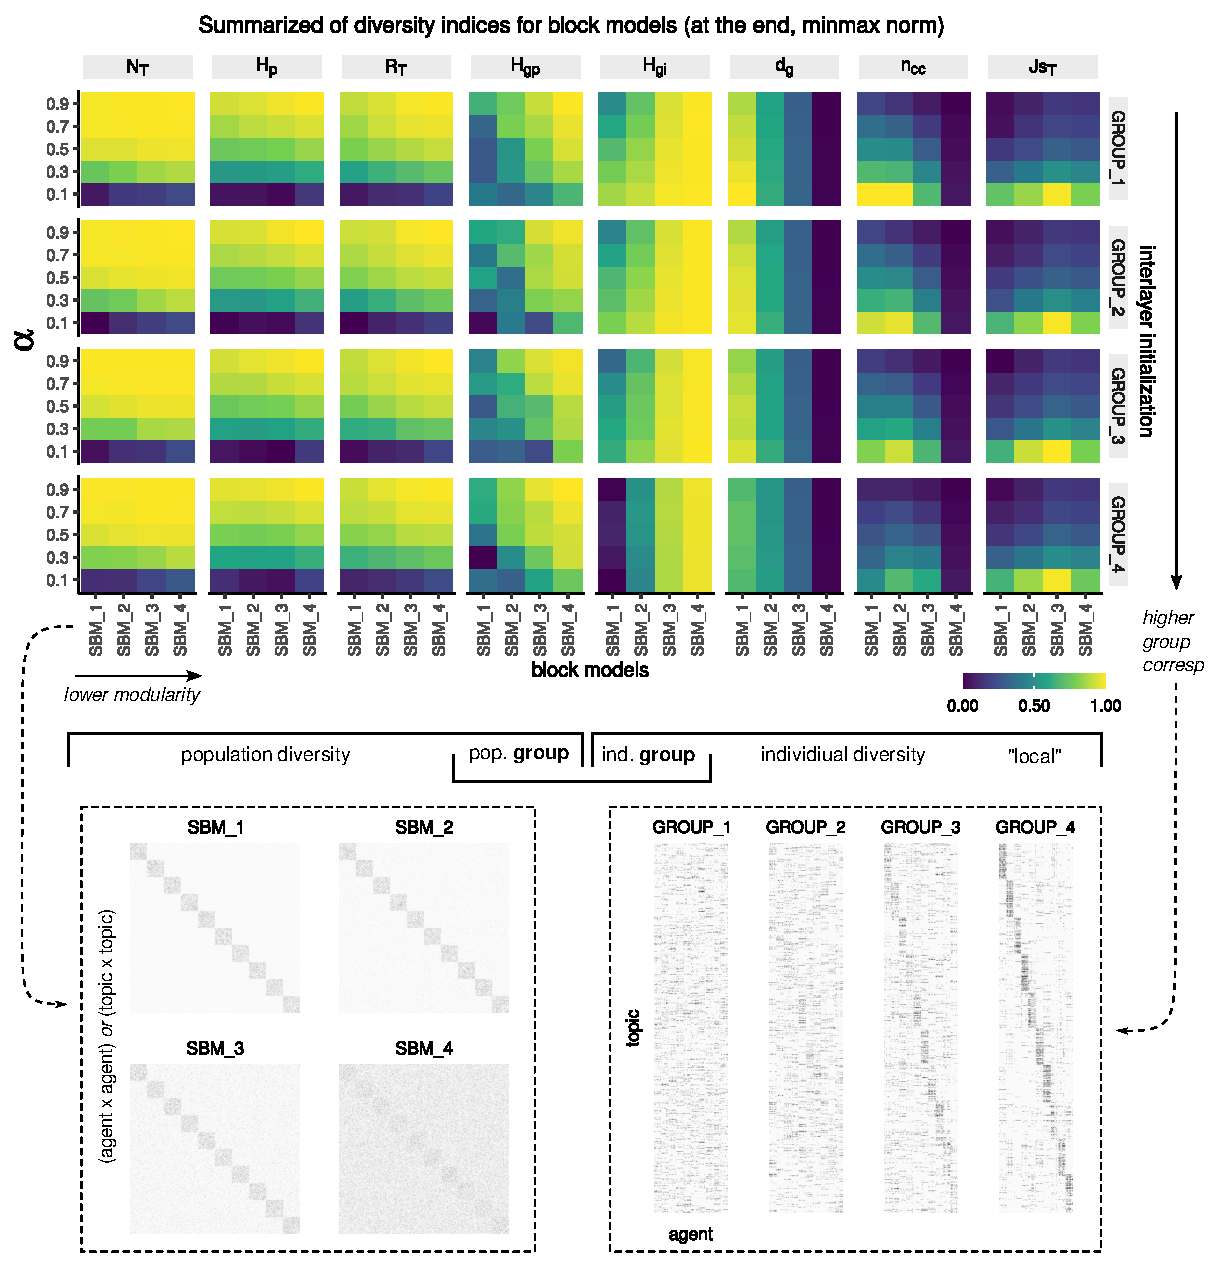
\includegraphics[width=\textwidth]{figures/Fig3.pdf}
    \caption{
    \textit{Summary  of  population  and  individual  diversity  indices  due  to $\alpha$,  across  different  block  models}. Within each heatmap, x-axis shows decreasing modularity of intralayer model (via increasing inter-modular connectivity), y-axis is $\alpha$. The color represents values at the end of the simulations, and min-max normalized within each metric. From left to right are different diversity metrics. From top to bottom are different group correspondence initialization strategies.
    }
    \label{fig:3}
\end{figure}
